\section{Ontology}
Choose Well defines its own RDF vocabulary. 
\todo[inline]{add figure number}
Fig. x contains the created ontology as a UML class diagram. 
The diagram uses these prefixes:
\todo[inline]{change font of prefixes to code}
\todo[inline]{add arrow symbols for prefixes}
\todo[inline]{add hashtags: /blob/main/choosewellHASHTAG http://www.w3.org/2000/01/rdf-schemaHASHTAG}
\begin{itemize}[noitemsep,nolistsep]
  \item cw: https://github.com/JiriResler/solid-choose-well-ontology/ \newline blob/main/choosewell for the Choose Well ontology.
  \item schema: \textbf{http://schema.org/} for the Schema.org general vocabulary. 
  \item rdfs: \textbf{http://www.w3.org/2000/01/rdf-schema} for the RDF Schema which provides a data-modelling vocabulary for RDF data.
  \item wikidata: \textbf{http://www.wikidata.org/entity/} for describing entities using the Wikidata knowledge base.
\end{itemize}

\begin{figure}[h]
  \centering
  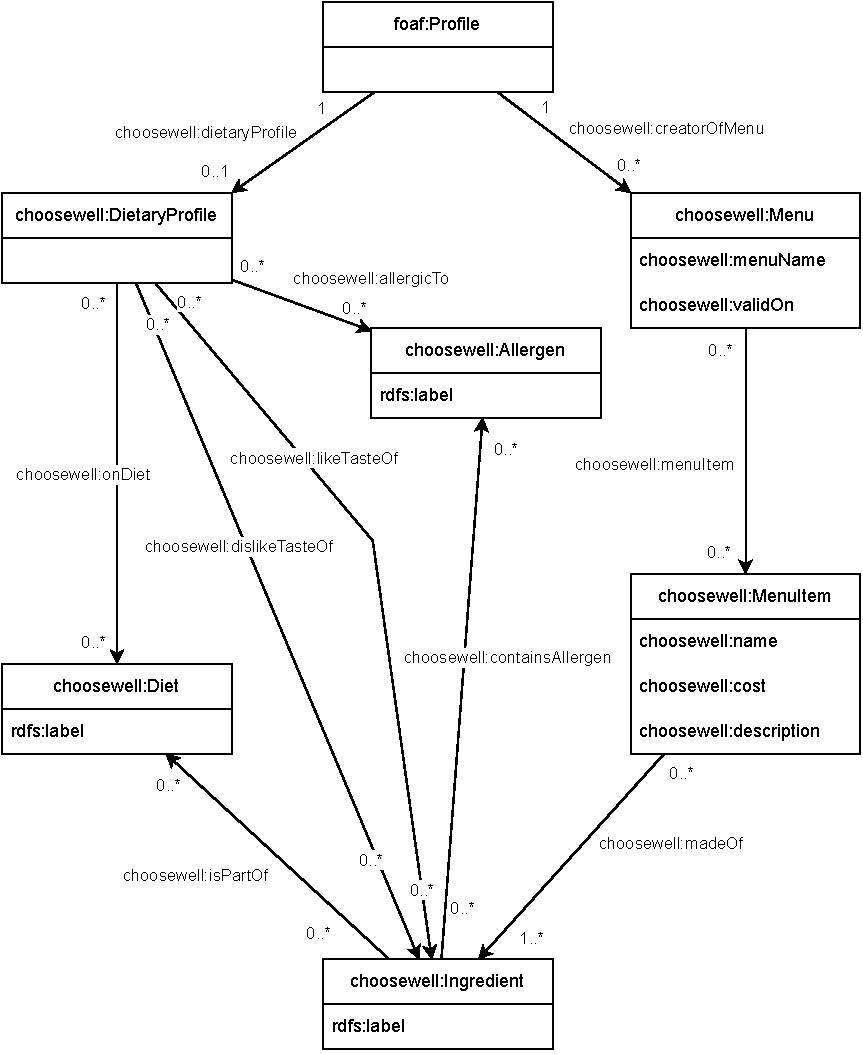
\includegraphics[width=\linewidth]{master-thesis/img/design-ontology.pdf}
  \caption{The Choose Well ontology}
\end{figure}